\documentclass[main.tex]{subfiles}
\begin{document}

\chapter{From a Lonely Road, to a Crowded Cluster}

\par \nar \rmsterope~watched in sadness as her family slowly drifted out of view.  A tear made of plasma streamed down the length of her face.  \rmsterope~ had a lonely road ahead.  But, little did she know, her isolation would not last for long.

\par \nar She drifted aimlessly through the Cosmos for several tens of thousands of years.  The scenery was nice for the most part, since she remained close to the disk of the Milky Way where most stars are currently being born.  The nebulae from which they are birthed are often beautiful to behold, illuminated by the light of the stars they birth.  A true symphony of color.  

\par \nar \rmsterope~  noticed that she happened to be moving in a very similar direction, with a very similar velocity, to a particularly far off but bright blob she couldn't quite resolve with the naked eye.  She could infer a rough distance based on having monitored her relative motion to it, however.\footnote{The term ``parallax'' refers to a technique used by astronomers to calculate the distances to the nearest objects to the Sun.  It is the angular separation on the sky between two independent measurements of an object's angular position, performed from two distinct locations with a large displacement or baseline.  The largest possible baseline is given by the motion of the Earth about the Sun, such that the two different measurements of the object's angular position are separated in time by $\sim$ 6 months, and the length of the corresponding baseline is twice the Earth's orbital distance from the Sun.  The basic idea behind the concept is most easily conveyed by extending one's arm outward in front, perpendicular to the torso.  Extend one finger in to the air and focus on it.  Close one eye.  Then close the other eye, and open the originally closed eye.  Repeat this process.  You will notice that your finger appears to suddenly shift positions relative to the background.  The scale of this shift depends on the relative distance between your eye and your finger, as well as between your finger and the background.  Hence, measuring the size of the angular displacement in degrees or radians can be used to compute the object's distance from the observer.  The concept is identical to that underlying stellar parallax. PICTURE OR DIAGRAM?}  It was far away and extended, no doubt about it.  Too big to be a star.  Too bright to be a few stars or even a gas cloud.  So what could it be?  That doesn't leave much...
%NL: Maybe we should define terms as ``basic'' as ``velocity'', as in the above?  But I am guessing this is not its first appearance...

\begin{figure}
\includegraphics[width=\columnwidth,angle=270,origin=c]{ch4_1.pdf}
\caption{\rmsterope~ noticing a fuzzy blob far off in the distance.  As she will soon discover, she is looking at an unresolved globular star cluster.  Illustration by Andre Pipe Oliva.
\label{fig:fig1}}
\end{figure}



\par \nar As the days, weeks, months, years and centuries passed, the far off blob drifted ever closer, occupying a larger and larger fraction of \rmsterope's view of the sky.  Regardless, the blob eluded resolution for what seemed to \rmsterope~ like a very long time.  But it continued to draw closer....
%NL: What about words like ``resolution''?  This seems a little high-level for early high school and younger.  Crap.  I guess we need to formally decide on a level of education to aim at, and go from there.  Just hoping to flag stuff like this for later...

\section{A New Home...?}

\par \nar One day, \rmsterope~  awoke surrounded by stars.  There were thousands, perhaps millions, within her immediate view.  She suddenly recalled drifting ever closer to something bright and blurry that she had never quite been able to see before falling asleep.  If her rough calculations were right, she was about due for a very close encounter with whatever the bright blurry object happened to be.  To her surprise, the mysterious object turned out to be a compact very dense cluster of stars; before awakening she had inadvertently wandered right in to the middle of it.\footnote{As was the case for the Seven Sisters, most, if not all, stars are thought to be born in "clusters", gravitationally-bound and compact groupings of stars, ranging in numbers from a few tens to several million, with central densities in the range 10 M$_{\odot}$ pc$^{-3}$ - 10$^6$ M$_{\odot}$ pc$^{-3}$.  These stars are all thought to form from the same Giant Molecular Cloud, as gravity shaped it into denser knots and filaments, creating the ideal environment for star formation.  However, the most massive star clusters, may be the products of the mergers of several lower mass clusters.  The answer to this question is still an active area of research.}

\par \nar The denizens of this cluster were typically old (i.e., billions of years in age), but the range of stellar ages was large; clearly, multiple episodes of stellar birth had occurred here at one time or another.  All together, a very large number of stars occupied a volume so compact the stellar density reached a million stars per cubic parsec at its center.\footnote{The field of the Milky Way, or No Man's Land, effectively denotes those regions in our Galaxy outside star clusters, the Galactic disk and its inner, denser central regions.  The Galactic field is where the stellar density is at its lowest in Our Galaxy, and the time for light to travel from one star to the next can be many many years. To put it into context, the Sun's nearest neighbor, Proxima Centauri, is located roughly one parsec away (or about 3.26 light years).  If you take the Sun and Proxima Centauri and place them in their current configuration in the star cluster currently hosting \rmsterope, roughly one hundred stars would lie between the pair.  \rmsterope's new home is a globular cluster, the oldest, most massive and densest of all star clusters.} 

\par \nar Obviously, traveling through the sparsely populated space of the Galactic field occupied the most time for any traveler, due its vast extent.  This is No Man's Land, a sea of now dead star-forming regions long forgotten, exhausted of their gas supplies.  Out in the Galactic halo and far from the disk\footnote{NEEDS A PICTURE, with a ``you are here'' showing the Sun. Point out the gas, star-forming regions, etc.} of the Galaxy where most stars are currently being born, only old massive and dense globular clusters exist, fossil records of a very early phase in the formation of the Galaxy.  Apart from these, stars are extremely scarce in these barren outer regions of our Galaxy. 

%NL: Adopt names of "old" people for the older stars:  i.e., Louise, Peggy, Daisy, Rose, Norma, etc.

\par \nar Suddenly, a strange voice interrupts \rmsterope~'s train of thought...

\par \Jane Hello there!  I see you are passing through in something of a hurry.  ...and there you go again.  Bye!

\par \nar \rmsterope~ realized she was moving a little faster than the other stars in the cluster.  Suddenly, she whipped past another one.

\par \Gene Hey!  Watch where you're going!

\par \Sterope So sorry!

\par \nar \rmsterope~ glanced back at the scene of the near-collision, grateful for those few kilometers that spared her from a direct collision.

\par \nar \rmsterope~ turned back around to face her forward motion, only to discover that she was about to collide with yet another star.  Frightened, she closed her eyes and hoped for the best.  

\par \Louise Whoa! Whoa! WHOA!

\par \nar It's a close call.  But the pair of stars manage to avoid a direct collision.  Instead, \rmsterope~ flies past \rmlouise, too fast to say hello.

\par \nar As \rmsterope~ whips by, her gravitational influence is felt by \rmlouise, and vice versa.  \rmsterope~ is more massive than the other stars in the cluster, since most are much older than her.  When she undergoes a close encounter with a much less massive \rmlouise, momentum conservation dictates that she induces a strong deflection to \rmlouise's trajectory through the cluster.\footnote{To remind the reader, the linear momentum of a particular is given by the product of its mass and velocity in 1D.  To change a particle's momentum, a net force must be applied for a finite interval of time.  Particles with more momentum require either a larger applied force or for a given force to be applied for a longer interval of time in order to significantly change their momentum.}  In this case, \rmlouise~ is flung off and escapes from the cluster, causing \rmsterope~ to end up gravitationally bound to it in \rmlouise's stead.  Momentum conservation strikes again!  Needless to say, \rmsterope~ felt terrible.

\par \Louise  AAAAAAHHHH!!! Help!  I'm floating away!

\par \Sterope I'm \textit{so} sorry!  I didn't mean to do it!  It was an accident.  

\par \Louise Uh...I don't think that helps me.  ...Nope, I'm still escaping to infinity.  This is all your faaauuullllttt...

\par \nar \rmsterope~ could barely hear \rmlouise~ now, as she retreated beyond the outer boundary of their host cluster and in to the empty space beyond, No Man's Land.

\par \Sterope WHAT?! I can't hear you?!?

\par \nar \rmsterope's shoulders slumped.  Another one bites the dust.  Saddened, she mutters defeatedly:

\par \Sterope I am more sorry than I could ever say.  Well... Good luck, I guess.  

\section{\rmsterope's New Neighbors}

\par \nar \rmsterope~ suddenly realized she was completely surrounded by stars.  They were so close she could make out the faces of hundreds, even thousands, of them.  This was a little too close for comfort for \rmsterope~, relative to what she had grown accustomed to over the last few million years.  In the neighborhood of the Sun, the approximate inter-stellar distance is of order one parsec.  Said another way, the distance between the Sun and its next nearest neighbor in the Galaxy, Proxima Centauri, is about one parsec (or about 3.26 light years).  Way out in the halo of the Galaxy, the Galactic field, No Man's Land, the inter-star distance drops by many orders of magnitude relative to the Solar neighborhood.  \rmsterope~ had been traveling for millions of years, a short span of time relative to her expected lifespan, but long enough for her to travel out of the Galactic Disk, and in to the Galactic Halo; a sparse sphere of old stars surrounding the Galactic Disk and Bulge.  Here, dense gravitationally-bound bundles of stars, called globular clusters, reside.  And not much else.

\par \nar \rmsterope~ was now in the very core of just such a globular cluster, having inadvertently collided with it while escaping from the Galaxy, via the Galactic Halo.  Gravity had acted to focus \rmsterope's trajectory, drawing her inward toward the million solar mass globular cluster.  Within the cluster core, the stellar density was now about a million times higher than in the Solar neighborhood; the average distance separating \rmsterope~ from her closest neighbor had gone from about a parsec, to about 1/100's of a parsec.  

\par \nar Startled and overwhelmed by all the staring faces, \rmsterope~ gasped.  It sure was a lot of personalities to introduce yourself to, get to know and, let's face it, tolerate.  \rmsterope~ wasn't so sure she was up for the job.

\par \Enrico Why hello there!  I am \rmenrico, it's nice to meet you.

\begin{figure}
\includegraphics[width=\columnwidth,angle=270,origin=c]{ch4_2.pdf}
\caption{\rmsterope~ as she meets \rmenrico~ for the first time.  Illustration by Andre Pipe Oliva.
\label{fig:fig1}}
\end{figure}

\par \nar \rmsterope~ turned suddenly, toward the mysterious voice.

\par \Sterope Uh...  Hi!  My name is \rmsterope.  If you don't mind me asking, where am I exactly?

\par \Enrico You find yourself in an old star cluster.  A globular cluster!  Most of the million or so stars spanning the roughly twenty parsecs of our cluster, where its outer reaches can be found, and where stars slowly bleed back in to No Man's Land, were born at more or less the same time as the rest of the older stars in the Galaxy.  From the same Mother Cloud.  I, on the other hand, am older and come from a different generation of stars.  

\par \Sterope All the stars are packed so close together here...

\par \Enrico Yep, it's crammed in here all right.  You get used to it pretty quickly though.  Mostly you don't notice it.  But, every now and then, two stars do smash in to each other.  They collide head-on.  BOOM!  More often though, two stars undergo strong deflections, during which one star passes by another star so closely that their stellar surfaces are almost touching.  Of course, if their surfaces don't touch, then instead of colliding they tend to bestow a strong deflection, one to the other.  This causes a deflection in each star's trajectory, and can either slow or speed them up.  

\par \Sterope Well, which is it?  Do they speed up or slow down?

\par \Enrico More massive stars tend to accelerate lower mass stars more easily, for a net gain of linear momentum.  Conversely, lower mass stars tend to \textit{be} accelerated by more massive stars such that, by conservation of linear momentum, the more massive perturbers tend to be decelerated. So, in the end, more massive stars tend to be slowed down, whereas lower mass stars tend to be sped up, on average.  Not much you can do about any of it, really, except enjoy the show...which by the way, I highly recommend.\footnote{An important thermodynamics-based analogy can be drawn between star clusters and a gas in a container.  The mean velocity of a star can be regarded as a proxy for its temperature:  larger mean motions imply hotter temperatures.  Since all particles in the system are free to interact and exchange energy (via mostly weak deflections induced by gravity in star clusters, and direct collisions between atoms or molecules in a gas), the system tends to evolve toward a "thermalized" state in which all particles have comparable kinetic energies or temperatures.}

\begin{figure}
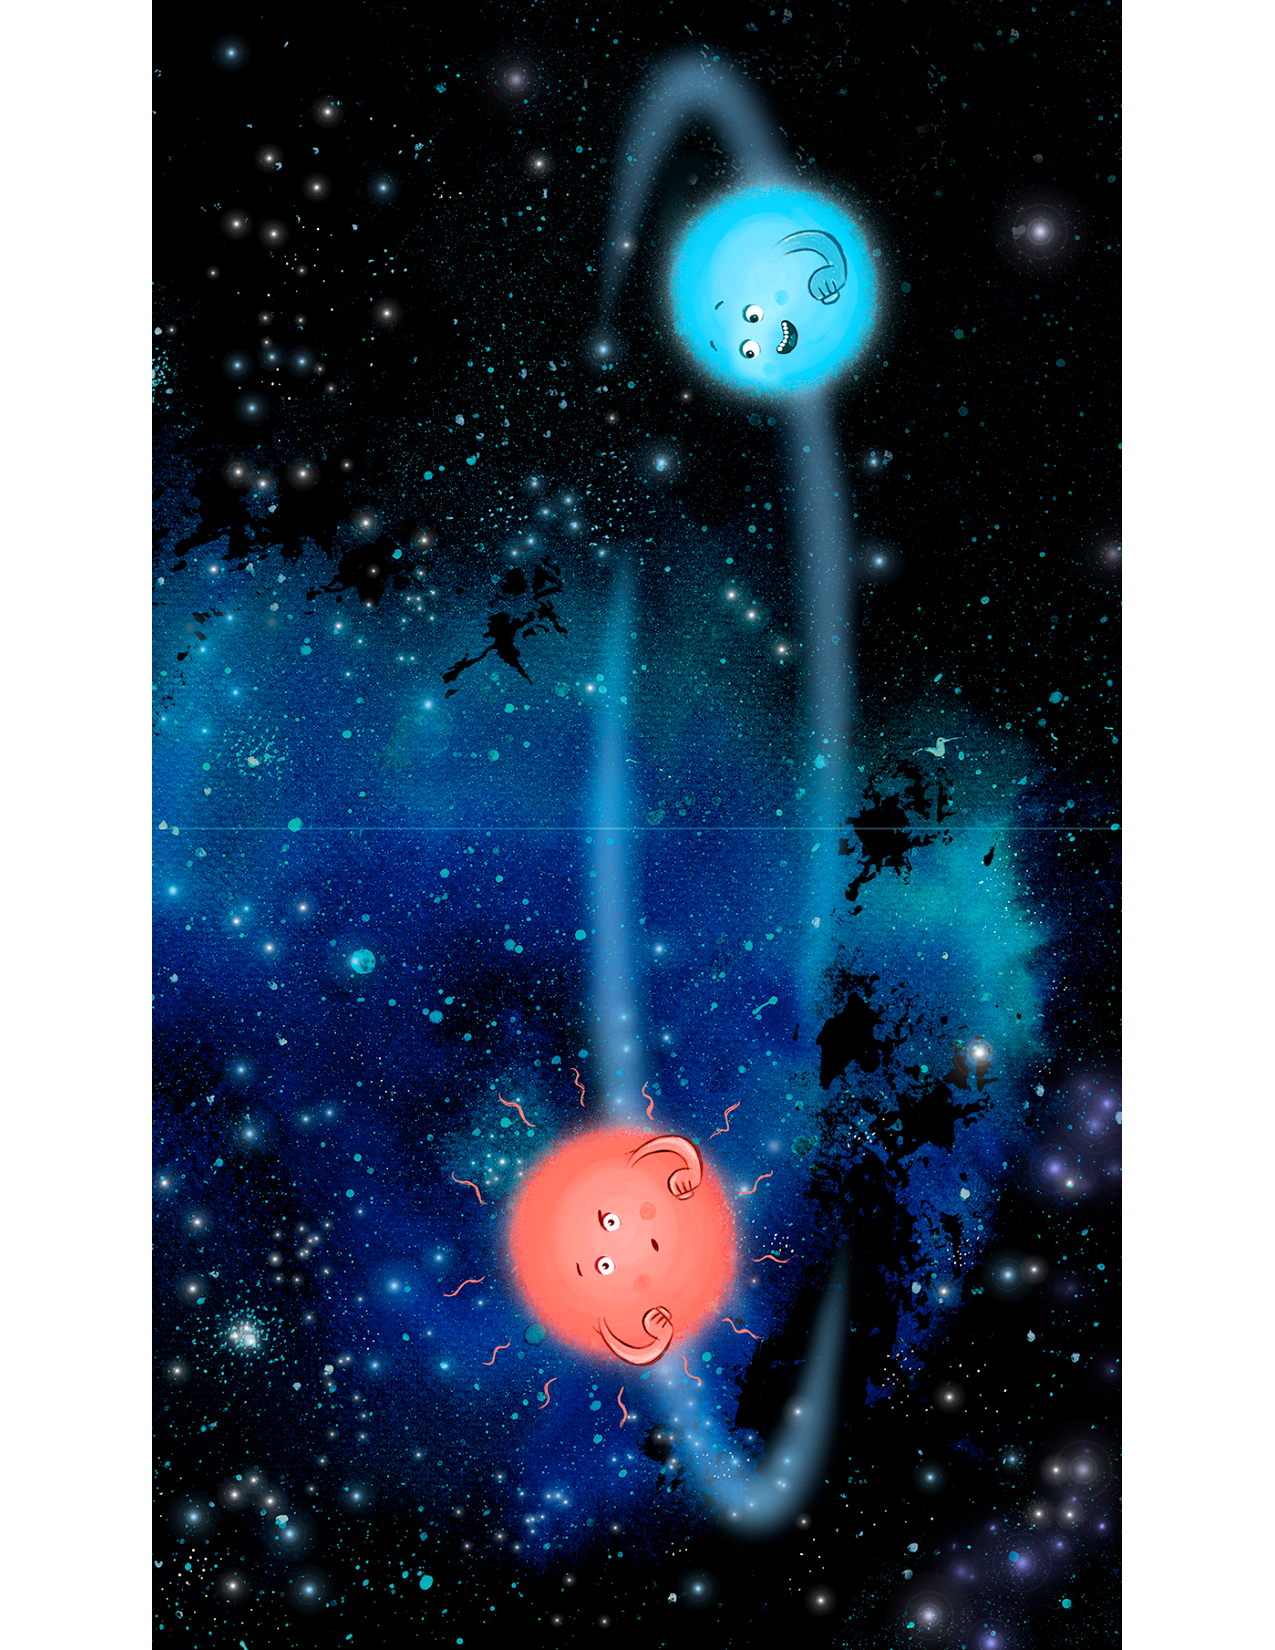
\includegraphics[width=\columnwidth,angle=270,origin=c]{ch3_3.pdf}
\caption{\rmenrico~ informs \rmsterope of what she must do in order to escape from the globular cluster she presently finds herself in.  Illustration by Andre Pipe Oliva.
\label{fig:fig1}}
\end{figure}

\par \nar \rmenrico~ winks at \rmsterope, who laughs.

\par \Sterope How old are you...if you don't mind me asking?

\par \nar \rmenrico~ thinks about the question for a moment...

\par \Enrico How old is the Universe now?  Wait...if I remember right, stars older than me used to yammer on about the number 13.7 Gyr for the age of the Universe, give or take a few hundred million years... I think...\footnote{All the available empirical data point to and are roughly consistent with this age for the Universe.  For example, no star older than this critical upper limit has ever been observed.}  Does that sound about right to you?

\par \Sterope I guess so, but I don't really know, to be honest.  I was not born long ago compared to you; it hasn't even been a billion years since my birth.

\par \Enrico You are a young one!  Good luck on all of life's many adventures, child.  

\par \Sterope Uh... Thanks?

\par \nar Suddenly and without warning, plasma shot out of \rmenrico's surface, below his equator.  A coronal mass ejection!\footnote{A coronal mass ejection (CME) refers to the ejection of plasma from the surface of a star.  Large amounts of matter (made up of protons and electrons, mostly) and electromagnetic radiation are launched out into space, and can either remain close to the stellar surface or be flung into the Solar System and beyond.  CMEs are known to be associated with very energetic shifts and changes in the star's outer magnetic field and a reorganization of its magnetic field lines.}  An old star, convective cells toiled at \rmenrico's surface, stirring upward the plasma from deep within his belly.  The plasma hit \rmenrico's photosphere\footnote{The photosphere is the outer shell of a star from which light is radiated and emerges.} with enough force to escape, drawing on the outward force supplied by nearby magnetic field lines.  Another explosion of plasma emerged from \rmenrico's lower hemisphere, not unlike a volcano erupting.

\par \Enrico My apologies!  This old star is at the mercy of surface convection!\footnote{If a steep enough temperature gradient (i.e., the temperature increases rapidly with increasing distance from the star's center of mass) exists in the interior of a star, an instability can arise in which heated plasma ascends and cooled plasma descends. This can also occur if the gas has a high heat capacity, implying that it cools slowly as it expands.  As a bubble of gas ascends, it finds itself in a region of lower pressure, allowing it to expand and cool.  The bubble must remain cooler and less dense than its surroundings in order to remain buoyant and continue to ascend.  Otherwise, if the bubble cools below the temperature of the new ambient plasma, its density will rise above that of the surrounding plasma and it will lose its buoyancy, sinking back down.}

\par \Sterope Oh, that's quite alright.  It could happen to anybody.

\par \Enrico Back to the question at hand.  Okay, so if the Universe is a little less than 14 billion years old, that must make me...twelve and a half billion years old?  Yep, that's the number!  Most of these other stars are more like nine billion years old...give or take a billion years or so.  Young pups, and they mostly keep to themselves.  I'm sorry if they seem rude but, in fairness, over 90\% of this cluster is comprised of their generation, so I guess it's no surprise they mostly keep to themselves.  

\par \Sterope Actually, I'm a little relieved.  This is a \textit{lot} of stars in a very crammed space.  I'm really not used to it, and was worrying how I would even begin getting to know all of these faces.

\par \Enrico Oh, don't worry about that.  I'm happy to chat any time you like, and to defer any time you prefer not to.  But these others will mostly inter-mingle with their own kind.  You'll be lucky if even one of them strikes up a serious conversation with you.  I mean, they are polite, I give them that.  They just prefer not to engage with outsiders directly, which are very rare around here.  You're the first one in well over a billion years!  

\par \Sterope Well, I'm perfectly fine with them keeping to themselves for the time being.  I think I will do the same... Hmmm... How do you suppose I might find my way out of here?

\par \Enrico You want out, huh?  I suppose I cannot blame you.  It is crowded in here.  But I warn you, accomplishing that feat is anything but easy.  Can I ask:  Where are you headed in such a hurry?

\par \Sterope Well, nowhere, really.  I guess I was just hoping to explore the Galaxy, and maybe even stumble across my missing siblings.  We were all born from the same Mother Cloud.  Ever since our birth cluster dispersed, I've been a little worried about them.  Now though, I'm more than a little worried that it's a really big Galaxy out there, and if they have been traveling as I have, then finding them within my lifespan could be impossible.  Still, I have to try!\footnote{SOMEWHERE IN THE BOOK, INCLUDE A MAP OF THE GALAXY, ALONG WITH ALL SEVEN SIBLINGS' PATHS THROUGHOUT IT!}

\par \Enrico Well, it sounds to me like you want to make your way back to the Galactic Bulge, which surrounds the central nuclear cluster and a non-negligible fraction of the Galactic Disk.  Unless I miss my guess, if you started out in the Galactic Disk somewhere, which is most likely the case for a young pup such as yourself, then your best bet for finding your siblings is in and around that central region of our Galaxy.  I know that doesn't narrow it down as much as you'd probably like, but at least it's a start.

\par \Sterope Thank you!  I really do appreciate it.  Yes, it is a \textit{definite} start.  Wait, just one more question:  How the heck do I get out of this cluster?

\par \Enrico Oh, right.  \textit{That} question.  Well, you're not going to like the answer.

\par \Sterope I don't care, try me anyway.

\par \Enrico To do that, you'll need to find not one, but \textit{two} black holes, lurking around somewhere here in the core.  I know they are here...somewhere.  

\par \Sterope Wait, what's a black hole?  And why do I need \textit{two} of them?

\par \Enrico Well, to answer the second question, you need \textit{mass} and \textit{lots of it} confined to a small volume if you want to be able to achieve the acceleration you will need to escape from this cluster.  This is a basic requirement in order for gravity to impart the required total force needed to achieve such a high velocity.  That is, a sufficiently large gravitational acceleration must be imparted over a given timescale in order to accelerate an object to a final velocity that exceeds the local escape velocity of the cluster.\footnote{The local escape velocity is defined as the minimum velocity required at a given distance from the cluster center of mass for the total energy of the escaper to exceed zero or, equivalently, to become gravitationally unbound.  A simple way to calculate the local escape velocity, using conservation of energy, is to equate the kinetic energy of an object to its local gravitational binding energy, keeping the object velocity as a free parameter.  If you solve this equation for the object velocity, you will obtain the minimum speed needed at that position in the host cluster gravitational potential for the object to become gravitationally unbound and escape to spatial infinity (asymptoting to zero velocity at spatial infinity in the context of this simple idealized equality).  PROVIDE EQUATIONS!!!} Looking at you, I'd guess you're, what, 3 maybe 4 solar masses?

\par \Sterope Whoa whoa WHOA!  My appearance is pretty much the last thing I wanted to discuss with you.  Besides, I really don't see how my weight is relevant to this discussion...

\par \Enrico Because I have some idea how massive the most massive black holes in this cluster might be, and you need \textit{two} that are each more massive than you.  The more massive they are relative to you, the easier it will be for you to achieve the required acceleration.

\par \Sterope Gotcha.  Alright, fine.  Last time I checked I was...

\par \nar \rmsterope's voice drops to a whisper...

\par \Sterope ...3.3 solar masses or so.  Buuuuuut I've burned through a lot of nuclear fuel since the last time I checked, so I think it's probably a bit less than that now.  

\par \Enrico Nothing to be ashamed of as far as I am concerned.

\par \Sterope Oh please, what do you weigh?  Half a solar mass?

\par \Enrico Nah, more like a quarter of a solar mass, last time I checked.\footnote{Stars in the main-sequence phase of lives share a relationship between their total mass and the duration of their lifespan spent on the main-sequence.  This relation is such that the most massive MS stars evolve the fastest, and have the shortest lifespans.  In fact, the evolution is so slow for the least massive MS stars that those with masses of only a few tenths of a solar mass should have total ages that exceed the current age of the Universe.  That is, some of these stars have been burning hydrogen into helium in their cores for over 13 billion years, and they are not yet done!}

\par \Sterope I am so jealous right now.  Alright, so what are these ``black holes'' you speak about, and how do we find them?

\par \Enrico Well, I guess the most important thing to know is that they are as dark as they come.  They don't shine.  At all.  So finding them is obviously a pretty serious challenge.  As to what they are, technically, they are the corpses of stars once much more massive than yourself, now wandering unseen through the Cosmos.

\par \Sterope  Dead stars?  Really?  So, basically, I am looking for ghosts haunting this cluster, which I rather conveniently cannot see?  And what is it you expect me to do with these dark ghosts, once I find them?

\par \Enrico You'll have to capture 'em.  Well, actually, first you'll have to convince two of them to partner up and form a bound binary system.  Then, you're going to need to convince them to let you take a run at them.  You'll have to work out the details on your own, which I warn you are not as straight-forward as you might expect, especially when chaos rears its ugly head and enters the picture.\footnote{The chaotic three-body problem has evaded a solution for centuries.  The reason is simple:  small perturbations to the initial conditions compound over time to change the very outcome of the interaction (e.g., which of the three particles is ejected).  A well known term for this is the "butterfly effect".}  But, in principle, two black holes bound in a compact binary should have enough binding energy to give you the acceleration you need to escape the cluster.\footnote{Recall that the binding energy of a binary star defines its internal reservoir of \textit{negative} energy.  The more negative the binary binding energy, the closer are the companions (for a given pair of companion masses).  Liouville's Theorem tells us that the total volume in phase space is conserved during the time evolution of self-gravitating N-body systems.  In practice, what this means is that the more negative the total energy, the more likely it is particles will be accelerated to high velocities.  Thus, it is easier for binaries with more binding energy to accelerate interloping single stars to above the local escape velocity of the host star cluster, even deep in the cluster core where the escape velocity is at its highest.}    

\par \Sterope Wow, that is a \textit{super} complicated plan.  Sigh.  Well, I guess I'll have to find a way to make it work, which brings me to my last question:  How, in the name of Hell, do I find these black holes?

\par \Enrico There is only one sure fire way, child.  You must search for a star orbiting within what appears to be a companion-less binary star system.  If the black hole forms a binary star system with another luminous star, \textit{any} luminous star, then it becomes possible to observe a star in orbit about something that cannot be seen.  This immediately implies the unseen presence of a dark compact object (i.e., a dead star) binary companion.  You can then use the orbital speed of the luminous companion as a function of distance from the unseen black hole to calculate the approximate mass of the black hole.  Just measure the time it takes the luminous companion to orbit the black hole once, and measure the distance from the center of mass that the companion appears to be orbiting.  The orbit should trace out an ellipse.  Calculate the typical orbital velocity by dividing the circumference of this circle by the orbital period.

\par \Sterope Wooooooooow.  This sounds like a loooooot of work.  I don't know about this... I mean, what are black holes even like?  \textit{If} I can find not one, but \textit{two} of them, do you think they will agree to help me escape from this cluster?

\par \Enrico Hmmmm... A fair and good question.  Few stars have gotten to really know a black hole and survived to tell the tale, to be honest with you... But they do have one weakness:  they have a constant hunger to grow.  Perhaps if you have food to offer in exchange for their services, they would be more inclined to help you out.  

\par \Sterope  So...bribery?  You are suggesting that I bribe them?  

\par \nar \rmenrico~ shrugs rather non-chalantly.

\par \Enrico It often works, I have to say.

\par \Sterope With what?

\par \Enrico Uh, well, mass.  Any mass will do.

\par \Sterope Okay...Again though, with what?

\par \Enrico Other stars?

\par \Sterope WHAT?! You want me to deliver other stars to these black holes so that they can eat them?  And the stars will die?

\par \Enrico No! No! I was just saying such a scenario \textit{could} work, at least in principle.  But, yes, those stars would surely die.  There are other options though!  Murder is not the only one.  Any mass will do.  The more of it you have, the better your position to bargain.  You could even trade some of your own mass in exchange for a boost!

\par \Sterope Okay, okay. So the mass could just as easily be the random crud out in No Man's Land?  

\par \Enrico I suppose so, yes.  Provided somebody could collect it all in to one place.

\par \Sterope So I could even take it from my own belly, or that of some other star?  Like, leave them alive, but take a little bit of their mass?

\par \Enrico I think that will work.  Good idea!

\par \Sterope Alright.  Now we're getting somewhere.  ...Wait, how do you suppose I collect mass?

\par \Enrico Off the top of my head, by finding those stars on the verge of evolving off the main-sequence\footnote{During the main-sequence (MS), stars are converting hydrogen into helium in their cores.  This is their primary source of energy, and makes them shine.  The MS is the first phase in the lifetime of a star, right after the protostellar phase.  It also tends to be the longest phase in the lifetime of a star, often lasting many hundreds or even thousands of times longer than later phases (e.g., the red giant branch phase).} and somehow getting your self close enough to them (i.e., in a binary system) that, when they evolve off the main-sequence and expand to become red giants\footnote{Red giant branch stars (RGB) are more evolved than MS stars, converting hydrogen into helium outside the core in a shell.  During the red giant branch phase, stars can expand by up to a factor of several hundred times their former size on the MS.  The outer envelope is only tenuously bound, and can easily be stripped by a binary companion as the star expands.}, they transfer the mass in their expanded envelope over to you.

\par \Sterope  Uh...Okay, so basically I am going to have to somehow figure out a way to swap myself in to \textit{and} out of at least one normal stellar binary system...in addition to two black hole binaries?  Then, I can use the mass of the black holes to accelerate me to above the escape speed from the cluster?  Just trying to wrap my head around this.  That seems like a lot of work.  Hmmmmm... Where do I even begin?

\par \Enrico Well, child, by my calculations, you need to participate in at least ten direct dynamical interactions with other singles or binaries in the cluster.  Two things can help with that:  increasing your mass, and reducing your velocity relative to the cluster average.  Both of these increase the rate of collisions with other stars or binaries in the cluster.\footnote{A simple estimate for the rate of direct collisions between identical single stars in a star cluster, borrowed from chemistry by considering a particle traveling through a uniform gaseous medium, comes from the mean free path (MFP) approximation.  Crudely, the MFP can be estimated by dimensional analysis, such that the mean free path l is l $\sim$ 1/n$\sigma$, where n is the mean particle number density and $\sigma$ is the collisional cross-section (i.e., an area corresponding to the direct overlap of two stars' radii; if a star passes within this area, a collision occurs).  If the mean particle velocity is v, then the rate of direct collisions is $\Gamma \sim$ n$\sigma$v and the mean time between collisions is $\tau \sim$ 1/$\Gamma$.}  The reason is related to something called gravitational focusing.  During the encounter, gravity helps out a lot; it serves to focus inward the relative trajectories of two colliding particles, making it so that they are more likely to collide.  Hence, slower incoming singles are more likely to collide directly with a binary due to this gravitational focusing, whereas without gravity it would not occur.\footnote{We are typically used to thinking of the collisional cross-section simply as the geometric surface area corresponding to the radii of two particles overlapping at closest approach.  That is, if the particle radius is R, n the geometrical cross-section for collision is $\pi$R$^2$.  The geometric cross-section can be enhanced when gravity is at work, and its effects in altering the velocities and trajectories of the interacting particles are non-negligible.  This new cross-section, called the gravitationally-focused cross-section for collision, can be calculated using conservation of energy and angular momentum. FINISH USING LEONARD OR SPITZER PAPERS.}

\par \Sterope Okay, got it...I think.  So...what do I do now?

\par \Enrico Not much you can do, but wait.  Don't worry though, gravity will do all the work for you.  It will carry you throughout this cluster, and deliver you close to other stars and binaries.  You are most likely to run in to the most massive objects in the cluster first; more massive objects exert the strongest gravitational force and, without even intending to, draw you in from further afar.  But massive objects are rare, and low-mass stars make up the vast majority of this old star cluster.  Usually the end result of these interactions is only a close approach, but often the encounter will be direct and you will become at least temporarily gravitationally bound to these other objects in the cluster...as you will find out for yourself soon enough!  

\par \nar \rmsterope~ noticed she had been drifting farther away from \rmenrico~.  She realized the process would continue, and they would soon part ways.

\par \Sterope I notice I am drifting away from you.  I can barely hear you anymore, in fact.  Thank you so much, \rmenrico, for all your help.  I'm off to find those two massive black holes!

\par \Enrico Good luck, young one.  It will take some time, but I have no doubt you will realize your goal of escaping eventually.

\begin{figure}
\includegraphics[width=\columnwidth,angle=270,origin=c]{ch4_4.pdf}
\caption{Armed with a satisfactory escape plan, \rmsterope~ drifts away from \rmenrico~, off in search of a couple black holes.  Illustration by Andre Pipe Oliva.
\label{fig:fig1}}
\end{figure}

\par \nar \rmsterope~ began her long journey through the cluster.  A sea of faces came in to and faded out of view.  One thing quickly became apparent to \rmsterope~ about her temporary neighbors:  they were highly skilled at avoiding eye contact.  So she continued on, mostly in silence, in search of the two massive black holes whose help she sought.

\end{document}


